\documentclass[conference]{IEEEtran}
\usepackage{amsmath,amssymb}
\usepackage{graphicx}
\usepackage{booktabs}
\usepackage{url}
\usepackage{tikz}
\usetikzlibrary{arrows.meta,positioning}
\graphicspath{{../figures/}{figures/}}

\begin{document}

\title{Do Zero-Shot Time-Series Foundation Models Detect Change Points? Forecast-Residual and Embedding-Distance Detectors vs.\ Classical CPD on Real-World and Industrial Sensor Data}

\author{\IEEEauthorblockN{Srikar}
\IEEEauthorblockA{\textit{Department and institution to be filled in}}}

\maketitle

\begin{abstract}
Time-series foundation models (TSFMs) forecast unseen series without any training, and their forecast error has been observed to spike when a signal changes. We test whether this makes them zero-shot change point detectors. We propose a forecast-residual detector that scores each time step by its one-step-ahead forecast surprise relative to the model's own predictive interval, built on Chronos-2 and TimesFM-2.5. We compare it with a split-window Chronos-2 embedding detector and with PELT, Binary Segmentation and BOCPD. Evaluation follows the TCPDBench protocol (multi-annotator F1 and segmentation covering, in default and oracle settings) on the 36 real-world series of the Turing Change Point Dataset and the 34 labelled files of the SKAB industrial testbed, and our baselines reproduce TCPDBench's published scores. With parameters fixed in advance, the Chronos-2 residual detector reaches a mean F1 of 0.668 on TCPD. Only Binary Segmentation scores higher (0.686), and the difference is not significant (Wilcoxon test, Holm-corrected $p=0.74$). The detector is strongest on short and medium-length series and weak on series of 512 points or more. When every method is tuned per series, the classical methods are significantly better on both datasets. On SKAB, no detector beats reporting no change points under F1. Zero-shot TSFMs are therefore a usable training-free change point detector, but not a replacement for tuned classical methods.

\end{abstract}

\begin{IEEEkeywords}
change point detection, time-series foundation models, zero-shot learning, Chronos-2, TimesFM, benchmark
\end{IEEEkeywords}

\section{Introduction}
Change point detection (CPD) finds the time steps at which the statistical behaviour of a time series changes, for example a shift in level, variance or dynamics. It is a basic step in monitoring industrial plants, finance and climate data. Classical methods such as PELT~\cite{killick2012pelt}, Binary Segmentation~\cite{scott1974binseg} and Bayesian online change point detection (BOCPD)~\cite{adams2007bocpd} are still the methods to beat on human-labelled benchmarks~\cite{vandenburg2020evaluation}. Learned detectors such as the time-invariant representation autoencoder (TIRE)~\cite{deryck2021tire} have to be trained for each new data source.

Time-series foundation models (TSFMs) such as Chronos~\cite{ansari2024chronos}, Chronos-2~\cite{ansari2025chronos2} and TimesFM~\cite{das2024timesfm} are pretrained on large forecasting corpora and can be used \emph{zero-shot}, without any training on the target data. Uray et al.~\cite{uray2026exploring} ran TimesFM zero-shot on the SWaT industrial testbed and observed that its forecast error spikes at the start and end of anomalous segments, and they name change point detection as a promising use of foundation models. They did not test this: their study has no change point metric, no CPD baseline and only one dataset. Choi et al.~\cite{choi2026nonstationarity} showed that Chronos-2 and MOMENT embeddings separate mean, variance and trend shifts, but only with supervised probes on synthetic AR(1) windows where the change is always in the middle.

This paper turns these observations into a direct test. Our research question is: \emph{can pretrained TSFMs, used zero-shot with no training, locate change points in real labelled data as accurately as established CPD methods?} We make the following contributions:
\begin{itemize}
\item A zero-shot \textbf{forecast-residual detector}: a one-step-ahead forecast surprise normalised by the model's own predictive interval, built on Chronos-2 and TimesFM-2.5. To our knowledge, this is the first evaluation of TSFM forecast residuals as a change point detector on labelled CPD benchmarks.
\item A simple \textbf{split-window embedding detector} on Chronos-2 for comparison. The idea of using frozen embeddings for CPD is concurrent work~\cite{anon2026gasfm}; we include it to compare the two ways of using a TSFM under one protocol.
\item An evaluation on the 36 human-annotated series of the Turing Change Point Dataset (TCPD)~\cite{vandenburg2020evaluation} and the 34 labelled files of the SKAB industrial testbed~\cite{skab}. We use the TCPDBench protocol (multi-annotator F1 and segmentation covering, default and oracle settings), and our classical baselines reproduce the published TCPDBench numbers.
\end{itemize}

\section{Related Work}
\textbf{Classical CPD.} PELT~\cite{killick2012pelt} and Binary Segmentation~\cite{scott1974binseg} minimise a penalised segmentation cost offline. BOCPD~\cite{adams2007bocpd} tracks a posterior over the current run length online. Truong et al.~\cite{truong2020ruptures} review offline methods and provide the \texttt{ruptures} library. TCPDBench~\cite{vandenburg2020evaluation} evaluated 14 methods on TCPD and found that simple methods remain hard to beat, and that a method returning no change points at all is a strong reference.

\textbf{Learned CPD.} KL-CPD~\cite{chang2019klcpd}, TS-CP2~\cite{deldari2021tscp2} and TIRE~\cite{deryck2021tire} learn representations in which a change becomes a large distance between neighbouring windows. TIRE, our IEEE base paper, trains an autoencoder whose time-invariant features are compared across adjacent windows. All of them must be trained on the target series. We ask whether a pretrained model can avoid this step. TIRE is discussed but not re-run, because its reference implementation carries no software license.

\textbf{TSFMs.} Chronos~\cite{ansari2024chronos} tokenises scaled values for a language-model backbone. Chronos-2~\cite{ansari2025chronos2} adds native multivariate input and quantile outputs. TimesFM~\cite{das2024timesfm} is a decoder-only patch transformer, and MOMENT~\cite{goswami2024moment} is a masked encoder aimed at representations. For anomaly detection, benchmarks such as TSB-AD~\cite{liu2024tsbad} use TSFM forecast or reconstruction errors as scores, and they find that TSFMs are often matched by simple methods. These studies score anomalous \emph{points or segments}, not change point locations.

\textbf{TSFMs and change points.} Uray et al.~\cite{uray2026exploring} motivate this work (Section~I). Choi et al.~\cite{choi2026nonstationarity} probe embeddings for the type of shift but do not localise it. A concurrent submission~\cite{anon2026gasfm} projects frozen TSFM embeddings to a univariate statistic and applies a statistical scan detector. Unlike these works, we study forecast residuals as well as embeddings, on real labelled CPD benchmarks, against classical CPD under the established TCPDBench protocol.

\section{Method}
Let $\mathbf{x}_{0:T}\in\mathbb{R}^{T\times C}$ be a series with $C$ channels, z-scored per channel. A detector outputs a set of change points $\hat{\mathcal{T}}\subset\{1,\dots,T-2\}$, each the first index of a new segment. Both TSFM detectors first produce a score $s_t$ for every time step and then share the same peak-picking step (Section~\ref{sec:peaks}), so differences between them come only from the scores. Fig.~\ref{fig:pipeline} summarises the pipeline.

\begin{figure}[t]
\centering
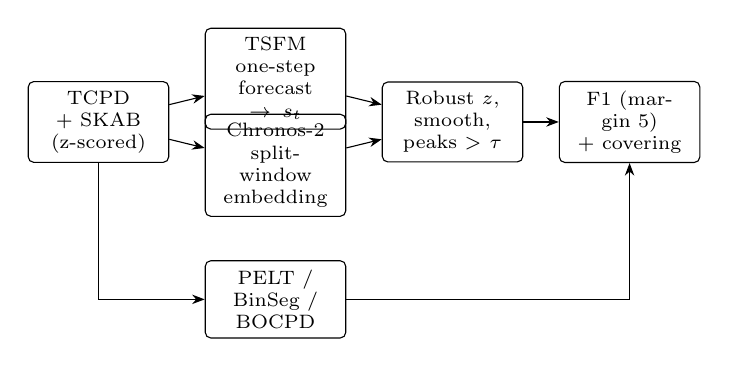
\begin{tikzpicture}[node distance=0.35cm and 0.45cm, every node/.style={font=\scriptsize, align=center},
  box/.style={draw, rounded corners=2pt, minimum height=0.75cm, text width=1.55cm}, >={Stealth[length=1.6mm]}]
\node[box] (data) {TCPD + SKAB\\(z-scored)};
\node[box, right=of data, yshift=0.55cm] (res) {TSFM one-step\\forecast $\to s_t$};
\node[box, right=of data, yshift=-0.55cm] (emb) {Chronos-2 split-\\window embedding};
\node[box, right=of res, yshift=-0.55cm] (pk) {Robust $z$, smooth,\\peaks $>\tau$};
\node[box, below=0.55cm of emb] (cls) {PELT / BinSeg /\\BOCPD};
\node[box, right=of pk] (ev) {F1 (margin 5)\\+ covering};
\draw[->] (data) -- (res); \draw[->] (data) -- (emb); \draw[->] (res) -- (pk); \draw[->] (emb) -- (pk);
\draw[->] (pk) -- (ev); \draw[->] (data) |- (cls); \draw[->] (cls) -| (ev);
\end{tikzpicture}
\caption{Pipeline. TSFM inference runs zero-shot on a Colab T4 GPU; everything else runs on a CPU.}
\label{fig:pipeline}
\end{figure}

\subsection{Forecast-residual detector}
For every $t$ the model forecasts $x_t$ one step ahead from the context $\mathbf{x}_{\max(0,t-L):t}$. The context grows from the start of the series until it reaches length $L$, so short series are still scored; steps with fewer than 8 past values get $s_t=0$. With predicted quantiles $\hat q^{0.1}, \hat q^{0.5}, \hat q^{0.9}$ the score is
\begin{equation}
s_t = \frac{1}{C}\sum_{c=1}^{C}\frac{\lvert x_{t,c}-\hat q^{0.5}_{t,c}\rvert}{\max\left(\hat q^{0.9}_{t,c}-\hat q^{0.1}_{t,c},\,\epsilon\right)},
\end{equation}
which is the surprise of the observed value relative to the model's own uncertainty, with $\epsilon=10^{-3}$. A change at $t$ makes $x_t$ unlike its context, so $s_t$ should peak at the first point of the new segment. Chronos-2 receives all channels jointly. TimesFM-2.5 is univariate, so each channel is forecast separately and the channel scores are averaged.

\subsection{Split-window embedding detector}
Chronos-2 normalises every input by its own mean and scale. If the windows before and after $t$ were embedded separately, a pure level shift would therefore disappear. Instead, we embed one window $\mathbf{x}_{t-w:t+w}$ centred on $t$ and take its patch-token embeddings $\mathbf{e}_1,\dots,\mathbf{e}_P$ (patch size 16, averaged over channels). With $\mathbf{h}^-_t$ and $\mathbf{h}^+_t$ the means of the left and right halves of the tokens,
\begin{equation}
d_t = 1-\cos\left(\mathbf{h}^-_t,\mathbf{h}^+_t\right).
\end{equation}
Both halves share one normalisation, so level and scale shifts remain visible. Steps closer than $w$ to either end get $d_t=0$.

\subsection{Shared peak picking}\label{sec:peaks}
Each score curve is robustly standardised as $(s_t-\mathrm{med}(s))/(1.4826\,\mathrm{MAD}(s))$ and smoothed with a centred moving average of width 3. Every local maximum above a threshold $\tau$, at least 5 steps from its neighbours, is reported as a change point.

\subsection{Classical baselines}
PELT and Binary Segmentation (\texttt{ruptures}~\cite{truong2020ruptures}) use a Gaussian mean-change cost. With the MBIC penalty ($3\log n$ plus $\log$ of each segment length), they reproduce the change points of the R \texttt{changepoint} defaults used by TCPDBench on all 32 univariate TCPD series. Binary Segmentation is capped at 5 change points by default, as in TCPDBench. BOCPD uses a Normal-Inverse-Gamma model with constant hazard $1/\lambda$. Our Python implementation follows the R \texttt{ocp} recursion, run-length truncation and MAP change point path, and returns the same change points as TCPDBench on all 36 TCPD series.

\section{Experimental Setup}
\textbf{Data.} TCPD~\cite{vandenburg2020evaluation} contains real series from economics, demography, climate, traffic and other domains, each annotated by five people. We keep the 36 series used in TCPDBench's averages: the five simulated quality-control series and \texttt{uk\_coal\_employ} (missing values) are excluded. SKAB~\cite{skab} contains 34 labelled files from a water-circulation Industrial-IoT testbed with 8 sensors sampled at about 1~Hz. The labelled change points mark the transitions into and out of induced faults. Table~\ref{tab:datasets} summarises both datasets. TCPD is short: half of its series have fewer than 275 points.

\begin{table}[t]
\centering
\caption{Datasets used (after TCPDBench's exclusions).}
\label{tab:datasets}
\resizebox{\columnwidth}{!}{%
\begin{tabular}{lrrrrrrrr}
\toprule
Dataset & Series & Multivariate & Length min & Length median & Length max & Annotators/series & Mean CPs/annotator & Margin \\
\midrule
TCPD & 36 & 4 & 15 & 274 & 991 & 5 & 2.46 & 5 \\
SKAB & 34 & 34 & 745 & 1140 & 1327 & 1 & 3.79 & 5 \\
\bottomrule
\end{tabular}
}
\end{table}


\textbf{Metrics.} We use the TCPDBench definitions~\cite{vandenburg2020evaluation}, ported verbatim and checked to reproduce TCPDBench's stored scores on all of its default runs.
\begin{itemize}
\item \emph{F1 with margin $M=5$.} Index 0 counts as a change point. Precision is computed against the union of all annotators, and recall is averaged over annotators.
\item \emph{Segmentation covering.} The covering of each annotator's segmentation by the predicted one~\cite{arbelaez2011contour}, averaged over annotators.
\end{itemize}
For SKAB (one annotator) we use the same margin. Its change points are at least about 55 steps apart, so the margins never overlap.

\textbf{Settings.} Following TCPDBench, every method is evaluated in two settings:
\begin{itemize}
\item \emph{Default}: one parameter set, fixed before any result was seen ($L=128$, $w=32$, $\tau=3$ for the TSFM detectors; package defaults for the baselines).
\item \emph{Oracle}: the per-series maximum over a parameter grid, an upper bound on what tuning could achieve.
\end{itemize}
The oracle grids are:
\begin{itemize}
\item PELT: 83 configurations (mean or mean-and-variance cost $\times$ 41 penalties).
\item Binary Segmentation: 165 configurations.
\item BOCPD: 501 configurations, the TCPDBench grid.
\item Residual detectors: 40 configurations ($L\in\{32,64,128,256\}\times$ 10 values of $\tau$).
\item Embedding detector: 30 configurations ($w\in\{16,32,64\}\times$ 10 values of $\tau$).
\end{itemize}
The TSFM grids are smaller, which can only lower their oracle scores. A method that returns no change points (\emph{Zero}) is reported as a reference.

\textbf{Implementation.}
\begin{itemize}
\item \emph{Models.} Chronos-2 (\texttt{amazon/chronos-2}, 120M parameters) and TimesFM-2.5 (\texttt{google/timesfm-2.5-200m-pytorch}) were loaded at pinned Hugging Face revisions. They ran zero-shot in fp32 on one NVIDIA T4 GPU in Google Colab (\texttt{chronos-forecasting} 2.3.2, \texttt{timesfm} 3.0.2, PyTorch 2.11).
\item \emph{Baselines.} The classical methods ran on a CPU.
\item \emph{Statistics.} Per-series F1 of each TSFM detector is compared with the best classical baseline using the Wilcoxon signed-rank test~\cite{wilcoxon1945} with Holm correction~\cite{holm1979}.
\end{itemize}
All code, configurations, the executed notebook and per-series results are released with the paper.

\begin{table}[t]
\centering
\caption{Reproduction of TCPDBench defaults on the 32 univariate TCPD series. PELT differs only by TCPDBench storing each change point one index early.}
\label{tab:tcpdbench}
\resizebox{\columnwidth}{!}{%
\begin{tabular}{lrrrr}
\toprule
Method & Ours F1 & TCPDBench F1 & Ours Cov & TCPDBench Cov \\
\midrule
Zero (no CPs) & 0.645 & 0.645 & 0.566 & 0.566 \\
BinSeg & 0.698 & 0.698 & 0.672 & 0.672 \\
PELT & 0.657 & 0.674 & 0.652 & 0.652 \\
BOCPD & 0.662 & 0.662 & 0.594 & 0.594 \\
\bottomrule
\end{tabular}
}
\end{table}


\section{Results}\label{sec:results}

\subsection{Reproduction of TCPDBench}
Table~\ref{tab:tcpdbench} compares our default-setting baselines with the scores stored by TCPDBench on the 32 univariate TCPD series. For Zero, Binary Segmentation and BOCPD, F1 and covering match to three decimals. PELT returns the same change points as the R \texttt{changepoint} run on every series. Its covering also matches (0.652). Its F1 is lower (0.657 vs.\ 0.674) only because TCPDBench stores each PELT change point one index early. Our metrics and baselines therefore reproduce the published benchmark, and the TSFM detectors below are scored on exactly the same footing.

\begin{table}[t]
\centering
\caption{Mean F1 (margin 5) and segmentation covering over series. Default: fixed parameters; oracle: best of each method's grid per series.}
\label{tab:main}
\resizebox{\columnwidth}{!}{%
\begin{tabular}{lrrrrrrrr}
\toprule
Method & TCPD default F1 & TCPD default Cov & TCPD oracle F1 & TCPD oracle Cov & SKAB default F1 & SKAB default Cov & SKAB oracle F1 & SKAB oracle Cov \\
\midrule
Zero (no CPs) & 0.638 & 0.554 & 0.638 & 0.554 & 0.349 & 0.364 & 0.349 & 0.364 \\
PELT & 0.652 & 0.640 & 0.864 & 0.772 & 0.147 & 0.248 & 0.512 & 0.754 \\
BinSeg & 0.686 & 0.665 & 0.861 & 0.774 & 0.347 & 0.621 & 0.463 & 0.727 \\
BOCPD & 0.656 & 0.578 & 0.892 & 0.785 & 0.185 & 0.369 & 0.559 & 0.699 \\
\bottomrule
\end{tabular}
}
\end{table}

\begin{table}[t]
\centering
\caption{Paired Wilcoxon signed-rank tests of per-series F1 against the best classical baseline of each dataset and setting (Holm-corrected over the three TSFM detectors).}
\label{tab:stats}
\resizebox{\columnwidth}{!}{%
\begin{tabular}{lrrrrrrr}
\toprule
Dataset & Setting & Detector & vs & Median diff & W/T/L & p & p (Holm) \\
\midrule
TCPD & default & Chronos-2 residual & BinSeg & -0.037 & 14/3/19 & 0.649 & 0.735 \\
TCPD & default & TimesFM-2.5 residual & BinSeg & -0.063 & 12/1/23 & 0.368 & 0.735 \\
TCPD & default & Chronos-2 embedding & BinSeg & -0.094 & 12/0/24 & 0.069 & 0.208 \\
TCPD & oracle & Chronos-2 residual & BOCPD & -0.038 & 9/6/21 & 0.006 & 0.012 \\
TCPD & oracle & TimesFM-2.5 residual & BOCPD & -0.033 & 11/5/20 & 0.016 & 0.016 \\
TCPD & oracle & Chronos-2 embedding & BOCPD & -0.132 & 5/7/24 & 0.000 & 0.000 \\
SKAB & default & Chronos-2 residual & BinSeg & -0.030 & 13/1/20 & 0.396 & 0.396 \\
SKAB & default & TimesFM-2.5 residual & BinSeg & -0.097 & 10/1/23 & 0.033 & 0.098 \\
SKAB & default & Chronos-2 embedding & BinSeg & 0.006 & 17/1/16 & 0.150 & 0.301 \\
SKAB & oracle & Chronos-2 residual & BOCPD & -0.119 & 4/5/25 & 0.000 & 0.000 \\
SKAB & oracle & TimesFM-2.5 residual & BOCPD & -0.213 & 1/7/26 & 0.000 & 0.000 \\
SKAB & oracle & Chronos-2 embedding & BOCPD & -0.238 & 5/3/26 & 0.000 & 0.000 \\
\bottomrule
\end{tabular}
}
\end{table}


\subsection{Default setting: zero-shot TSFMs vs.\ untuned classical CPD}
Table~\ref{tab:main} gives mean F1 and covering, and Fig.~\ref{fig:box} shows the per-series spread of F1 in the default setting.

\textbf{TCPD.} The Chronos-2 residual detector reaches a mean F1 of 0.668. It is second of the six detectors, behind Binary Segmentation (0.686) and ahead of BOCPD (0.656) and PELT (0.652). It also has the highest median per-series F1 of all methods (0.711). TimesFM-2.5 residual (0.641) is only just above Zero (0.638), and the embedding detector (0.605) falls below it. On covering, Binary Segmentation (0.665) and PELT (0.640) lead, ahead of Chronos-2 residual (0.608).

\textbf{SKAB.} No detector beats Zero under F1 (0.349). The best are Binary Segmentation (0.333) and Chronos-2 residual (0.303). Under covering, every detector except PELT scores above Zero (0.364). Binary Segmentation leads (0.616), followed by the embedding detector (0.575).

\textbf{Significance.} Binary Segmentation is the best classical method in the default setting on both datasets. Table~\ref{tab:stats} compares each TSFM detector with it. None of the three differs significantly from it on either dataset: all Holm-corrected $p\geq0.098$. On TCPD, Chronos-2 residual wins on 14 series, ties on 3 and loses on 19 (median difference $-0.037$, $p=0.735$). On SKAB, the embedding detector wins on slightly more series than it loses (17/1/16).

\begin{figure*}[t]
\centering
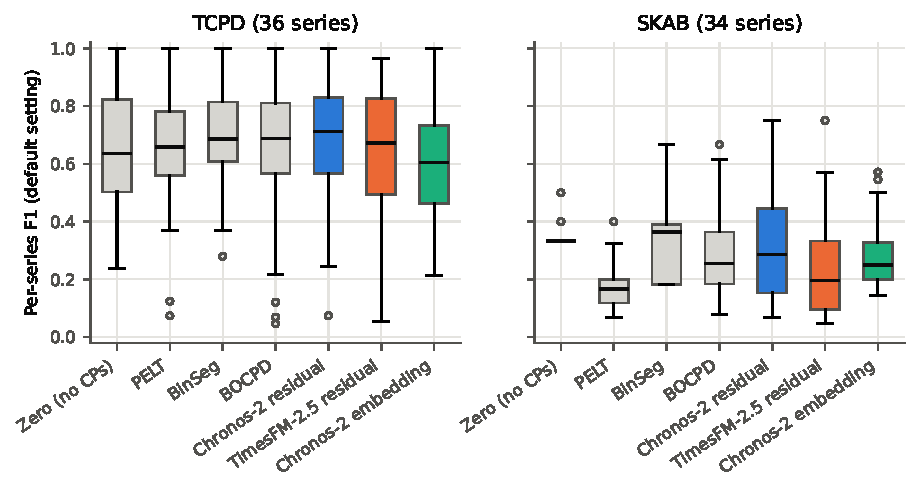
\includegraphics[width=0.85\textwidth]{fig3_f1_boxplot}
\caption{Per-series F1 in the default setting. TSFM detectors are coloured; classical methods and Zero are grey.}
\label{fig:box}
\end{figure*}

\subsection{Oracle setting}
Tuning per series raises every method, but the classical methods gain more (Table~\ref{tab:main}). BOCPD reaches 0.892 on TCPD, against 0.828 for Chronos-2 residual, 0.827 for TimesFM-2.5 residual and 0.739 for the embedding detector. On SKAB it reaches 0.634, against 0.477, 0.426 and 0.422. All six differences are significant after Holm correction: on TCPD $p=0.012$, $0.016$ and $<0.001$; on SKAB $p<0.001$ for all three (Table~\ref{tab:stats}).

The classical grids are larger (83--501 configurations against 40 for each residual detector), so we also cut every classical grid to 40 evenly spaced configurations. Oracle F1 drops only slightly:
\begin{itemize}
\item BOCPD: 0.871 on TCPD and 0.600 on SKAB;
\item PELT: 0.857 and 0.572;
\item Binary Segmentation: 0.855 and 0.526.
\end{itemize}
All of these remain above the best TSFM oracle (0.828 on TCPD, 0.477 on SKAB). The oracle gap is therefore not an artefact of grid size.

\subsection{Effect of series length}
We split the TCPD default F1 by series length into four groups:
\begin{itemize}
\item \emph{Shorter than 100 points (9 series).} BOCPD leads (0.833), followed by Chronos-2 residual (0.811) and TimesFM-2.5 residual (0.807). Both are well ahead of PELT and Binary Segmentation (0.727 each).
\item \emph{100--255 points (9 series).} Binary Segmentation (0.795) and PELT (0.758) lead, ahead of Chronos-2 residual (0.734) and TimesFM-2.5 residual (0.729).
\item \emph{256--511 points (10 series).} Chronos-2 residual is the best method (0.678), narrowly ahead of BOCPD (0.672) and PELT (0.671).
\item \emph{512 points or more (8 series).} Every detector falls below Zero (0.702). The lowest scores are TimesFM-2.5 residual (0.376), BOCPD (0.405) and Chronos-2 residual (0.421).
\end{itemize}
All SKAB files are longer than 512 points (745--1327).

\subsection{Context length and the first time steps}
Fig.~\ref{fig:context} shows mean F1 for each context length $L$ at the default $\tau=3$. On TCPD, F1 stays between 0.653 and 0.679 for Chronos-2 and between 0.639 and 0.668 for TimesFM-2.5. On SKAB, the longest context ($L=256$) is best for both models (0.322 and 0.281). The default $L=128$ was fixed in advance and is not the best on either dataset. The best $L$ would add 0.011 (Chronos-2) and 0.026 (TimesFM-2.5) to mean F1 on TCPD, and 0.019 and 0.038 on SKAB.

In its first steps, the residual detector forecasts from a very short context. To check whether this produces spurious detections, we set the scores of the first 32 steps to zero. SKAB F1 rises by less than 0.01 (0.303 to 0.308 for Chronos-2, 0.244 to 0.250 for TimesFM-2.5). TCPD F1 falls (0.668 to 0.627 and 0.641 to 0.618), because 15 of the 36 TCPD series have an annotated change point in their first 32 steps. The results are therefore not driven by an early-context artefact.

\begin{figure*}[t]
\centering
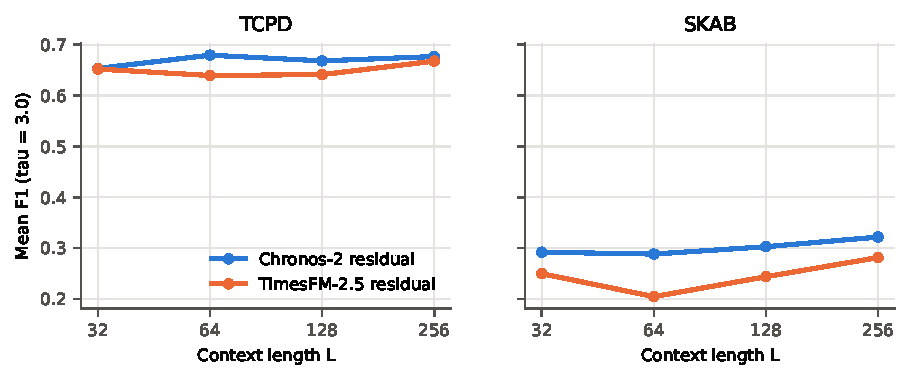
\includegraphics[width=0.85\textwidth]{fig4_context_length}
\caption{Mean F1 of the residual detectors against context length $L$ ($\tau=3$).}
\label{fig:context}
\end{figure*}

\begin{table}[t]
\centering
\caption{Mean runtime per series at default parameters. Classical methods: one CPU core; TSFM detectors: one Colab T4 GPU (model inference only).}
\label{tab:runtime}
\resizebox{\columnwidth}{!}{%
\begin{tabular}{lrr}
\toprule
Method & SKAB (s/series) & TCPD (s/series) \\
\midrule
BinSeg & 0.36 & 0.09 \\
BOCPD & 0.70 & 0.33 \\
Chronos-2 embedding & 6.59 & 0.30 \\
Chronos-2 residual & 11.41 & 0.51 \\
PELT & 2.91 & 0.49 \\
TimesFM-2.5 residual & 25.49 & 1.62 \\
\bottomrule
\end{tabular}
}
\end{table}


\subsection{Runtime}
Table~\ref{tab:runtime} reports the mean runtime per series in the default setting. On SKAB, the classical methods need 0.36\,s (Binary Segmentation), 0.70\,s (BOCPD) and 2.91\,s (PELT) on one CPU core. The TSFM detectors need 6.59\,s (embedding), 11.41\,s (Chronos-2 residual) and 25.49\,s (TimesFM-2.5 residual) on a T4 GPU, counting model inference only. The residual detector needs one forecast per time step. TimesFM-2.5 is the slowest, partly because it forecasts each of SKAB's 8 channels separately. The hardware differs, so these numbers show the order of magnitude rather than a like-for-like comparison.

\subsection{Qualitative example}
Fig.~\ref{fig:example} shows the TimesFM-2.5 residual score on two series. Both were chosen before any TSFM result was seen. On \texttt{nile}, the score peaks just after the annotated change, but the peak stays below $\tau=3$, so the default setting reports no change point. On \texttt{valve1\_0}, the score crosses $\tau$ many times away from the four annotated change points, including a very large spike in the first steps, where the context is shortest.

\begin{figure*}[t]
\centering
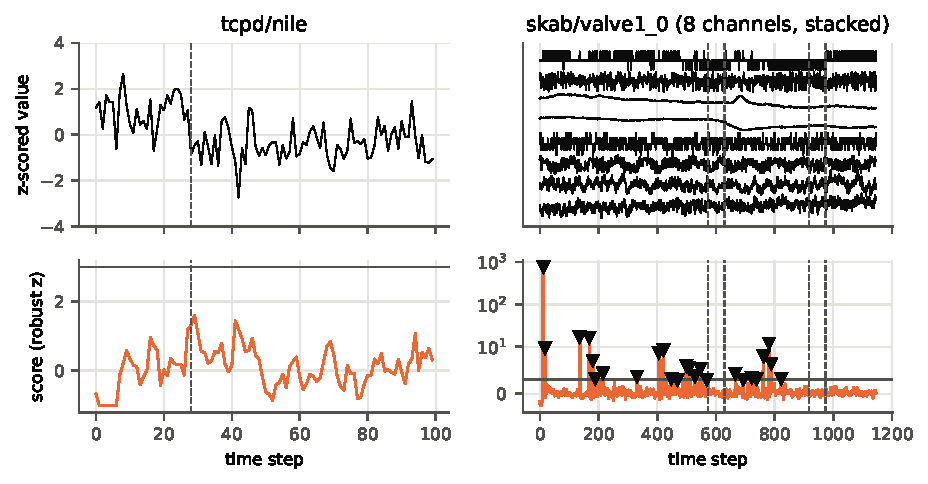
\includegraphics[width=0.85\textwidth]{fig2_example}
\caption{TimesFM-2.5 residual detector ($L=128$, $\tau=3$) on TCPD \texttt{nile} (left) and SKAB \texttt{valve1\_0} (right, 8 channels stacked). Top: z-scored series. Bottom: the standardised score that peak picking sees, with the threshold $\tau$ (solid line) and the detections (triangles). Dashed lines mark the annotated change points.}
\label{fig:example}
\end{figure*}

\section{Discussion}
\textbf{Answer to the research question.} Partly. With no training and no tuning, the Chronos-2 forecast residual locates change points about as well as untuned classical CPD on real-world data. It is statistically tied with the best classical method on TCPD and has the highest median F1 there. The observation of Uray et al.~\cite{uray2026exploring}, that forecast error spikes at changes, therefore holds up as a usable detector. It is not a replacement for classical CPD, though: once methods are tuned the classical ones are significantly better, and the TSFM detectors are weak on long series and on the industrial SKAB data.

\textbf{Where the TSFM detectors fail.} Fig.~\ref{fig:example} suggests a likely reason for the weak results on long and noisy multichannel signals. Such signals produce many short-lived forecast surprises that cross a fixed threshold: isolated spikes and the start of the series, where the context is shortest. A persistent change, by contrast, soon becomes part of the context, so its surprise is brief and may stay below $\tau$. Tuning cannot fully repair this. The classical methods expose parameters that directly control the segmentation (a penalty, or a hazard rate and priors), whereas the TSFM detectors expose only $\tau$ and $L$, and a per-series threshold cannot help when the largest score peaks are not at the change points. This reading is consistent with the oracle and length results, but we have not tested it directly.

\textbf{Residuals vs.\ embeddings, and Chronos-2 vs.\ TimesFM-2.5.} With the same model, the Chronos-2 forecast residual beats our embedding detector on F1 on both datasets (0.668 vs.\ 0.605 on TCPD, 0.303 vs.\ 0.272 on SKAB). A plausible reason is that the residual is normalised by the model's own predictive interval, whereas a cosine distance between embeddings has no natural scale. The embedding detector does segment SKAB better than the residual detectors under covering (0.575). This result concerns our simple split-window detector only; it says nothing about more elaborate embedding methods such as GAS-FM~\cite{anon2026gasfm}. Chronos-2 is ahead of TimesFM-2.5 on both datasets. The lead also holds on the 32 univariate TCPD series (0.680 vs.\ 0.650), so it is not only due to Chronos-2's joint multivariate input.

\textbf{Practical guidance.} When no labels are available for tuning and the series are short, a zero-shot TSFM residual detector is a reasonable training-free choice. When labels allow tuning, when series are long, or when compute is limited, classical CPD remains the better option.

\textbf{Limitations.}
\begin{itemize}
\item We test only two TSFMs, with a single fixed threshold for all series.
\item As in TCPDBench, the oracle setting is an upper bound on the same labels, not a held-out result.
\item SKAB has a single annotator, and its labels mark the start and end of induced faults, which are not always sharp statistical changes.
\item The TSFM and classical runtimes were measured on different hardware.
\item TIRE~\cite{deryck2021tire} was not re-run because its code has no license, and the concurrent GAS-FM method was not compared directly.
\end{itemize}

\section{Conclusion}
We tested whether pretrained time-series foundation models, used zero-shot, can locate change points in human-labelled data. We built a forecast-residual detector on Chronos-2 and TimesFM-2.5 and evaluated it under the TCPDBench protocol on TCPD and SKAB, with classical baselines that reproduce the published benchmark. Without any tuning, the Chronos-2 residual detector matches classical CPD on TCPD and is strongest on short and medium-length series. Tuned classical methods remain significantly better, and no method beats predicting no change on SKAB under F1. Future work includes adaptive, per-series thresholds, better use of multivariate input, more industrial datasets, and combining TSFM residual scores with classical segmentation.


\bibliographystyle{IEEEtran}
\bibliography{refs}

\end{document}
